% you need to build with xelatex
\documentclass[t,aspectratio=169]{beamer}

\usepackage{longtable}
\usepackage{tikz,multirow,array,colortbl,multimedia}
\usetikzlibrary{arrows,shapes,decorations.shapes,shadows,calc}
\usetikzlibrary{shapes.callouts, decorations.text}

\tikzstyle{flow}=[->, >=stealth', thick, shorten >=3pt, shorten <=3pt]
\usepackage{pdfpages}
\usepackage{times,amsmath,graphicx,marvosym}
\usepackage{multirow,array,colortbl,multimedia}
\usepackage{graphicx}
\usepackage{natbib}

\def\aaps{A\&AS}           % Astronomy and Astrophysics Suplement
\def\aap{A\&A}             % Astronomy and Astrophysics
\def\ssr{Space~Sci.~Rev.}  % Space Science Reviews
\def\apj{ApJ}              % Astrophysical Journal
\def\aj{AJ}                % Astronomical Journal
\def\mnras{MNRAS}          % Monthly Notices of the RAS
\def\araa{ARA\&A}          % Annual Review of Astron and Astrophys
\def\nat{Nature}           % Nature
\def\apjl{ApJ}             % Astrophysical Journal, Letters
\def\procspie{Proc.\ SPIE} % Proceedings of the SPIE
\def\pasp{PASP}

\def\degr{\hbox{$^\circ$}}
\def\arcmin{\hbox{$^\prime$}}
\def\arcsec{\hbox{$^{\prime\prime}$}}
\def\fs{\hbox{$.\!\!^{\rm s}$}}
\def\fdg{\hbox{$.\!\!^\circ$}}
\def\farcm{\hbox{$.\mkern-4mu^\prime$}}
\def\farcs{\hbox{$.\!\!^{\prime\prime}$}}
\def\sun{\hbox{$\odot$}}


\newcommand{\jira}[1]{\href{https://jira.lsstcorp.org/browse/#1}{#1}}

\newcommand{\bfvec}[1]{\mbox{$\bf#1$}}
\newcommand{\citell}{\citeyear}
\newcommand{\citeds}{\citeyear}
\newcommand{\citellp}{\citeyearpar}
\newcommand{\citedsp}{\citeyearpar}
\providecommand{\secref}[1]{Section~\ref{#1}}
\providecommand{\appref}[1]{Appendix~\ref{#1}}
\providecommand{\partref}[1]{Part~\ref{#1}}
\providecommand{\tabref}[1]{Table~\ref{#1}}
\providecommand{\figref}[1]{Figure~\ref{#1}}
\providecommand{\eqnref}[1]{Eq.~\ref{#1}}
\providecommand{\reqref}[1]{Req.~\ref{#1}}
\providecommand{\actref}[1]{AI~\ref{#1}}



\usepackage[backgroundTheme=LSST2017,
  fonts=false, colorlinks=false,
 footline={Project Comunity Workshop  $\bullet$ Tucson, AZ $\bullet$ August 12--15, 2019},
meeting={Project Comunity Workshop},
position={DM Project Manager}
]{LSST-beamer}
\usepackage{siunitx}
\usepackage{framed}


\title{LSST Data Management All Hands}
\date{12\textsuperscript{th} Aug 2019}

\author{William O'Mullane}
\institute{AURA/LSST}


\graphicspath{ {./figures} {./images/}  }



\begin{document}

\maketitle
\section{LSST}
\frame{\frametitle{ Site shaping up }
\begin{center}
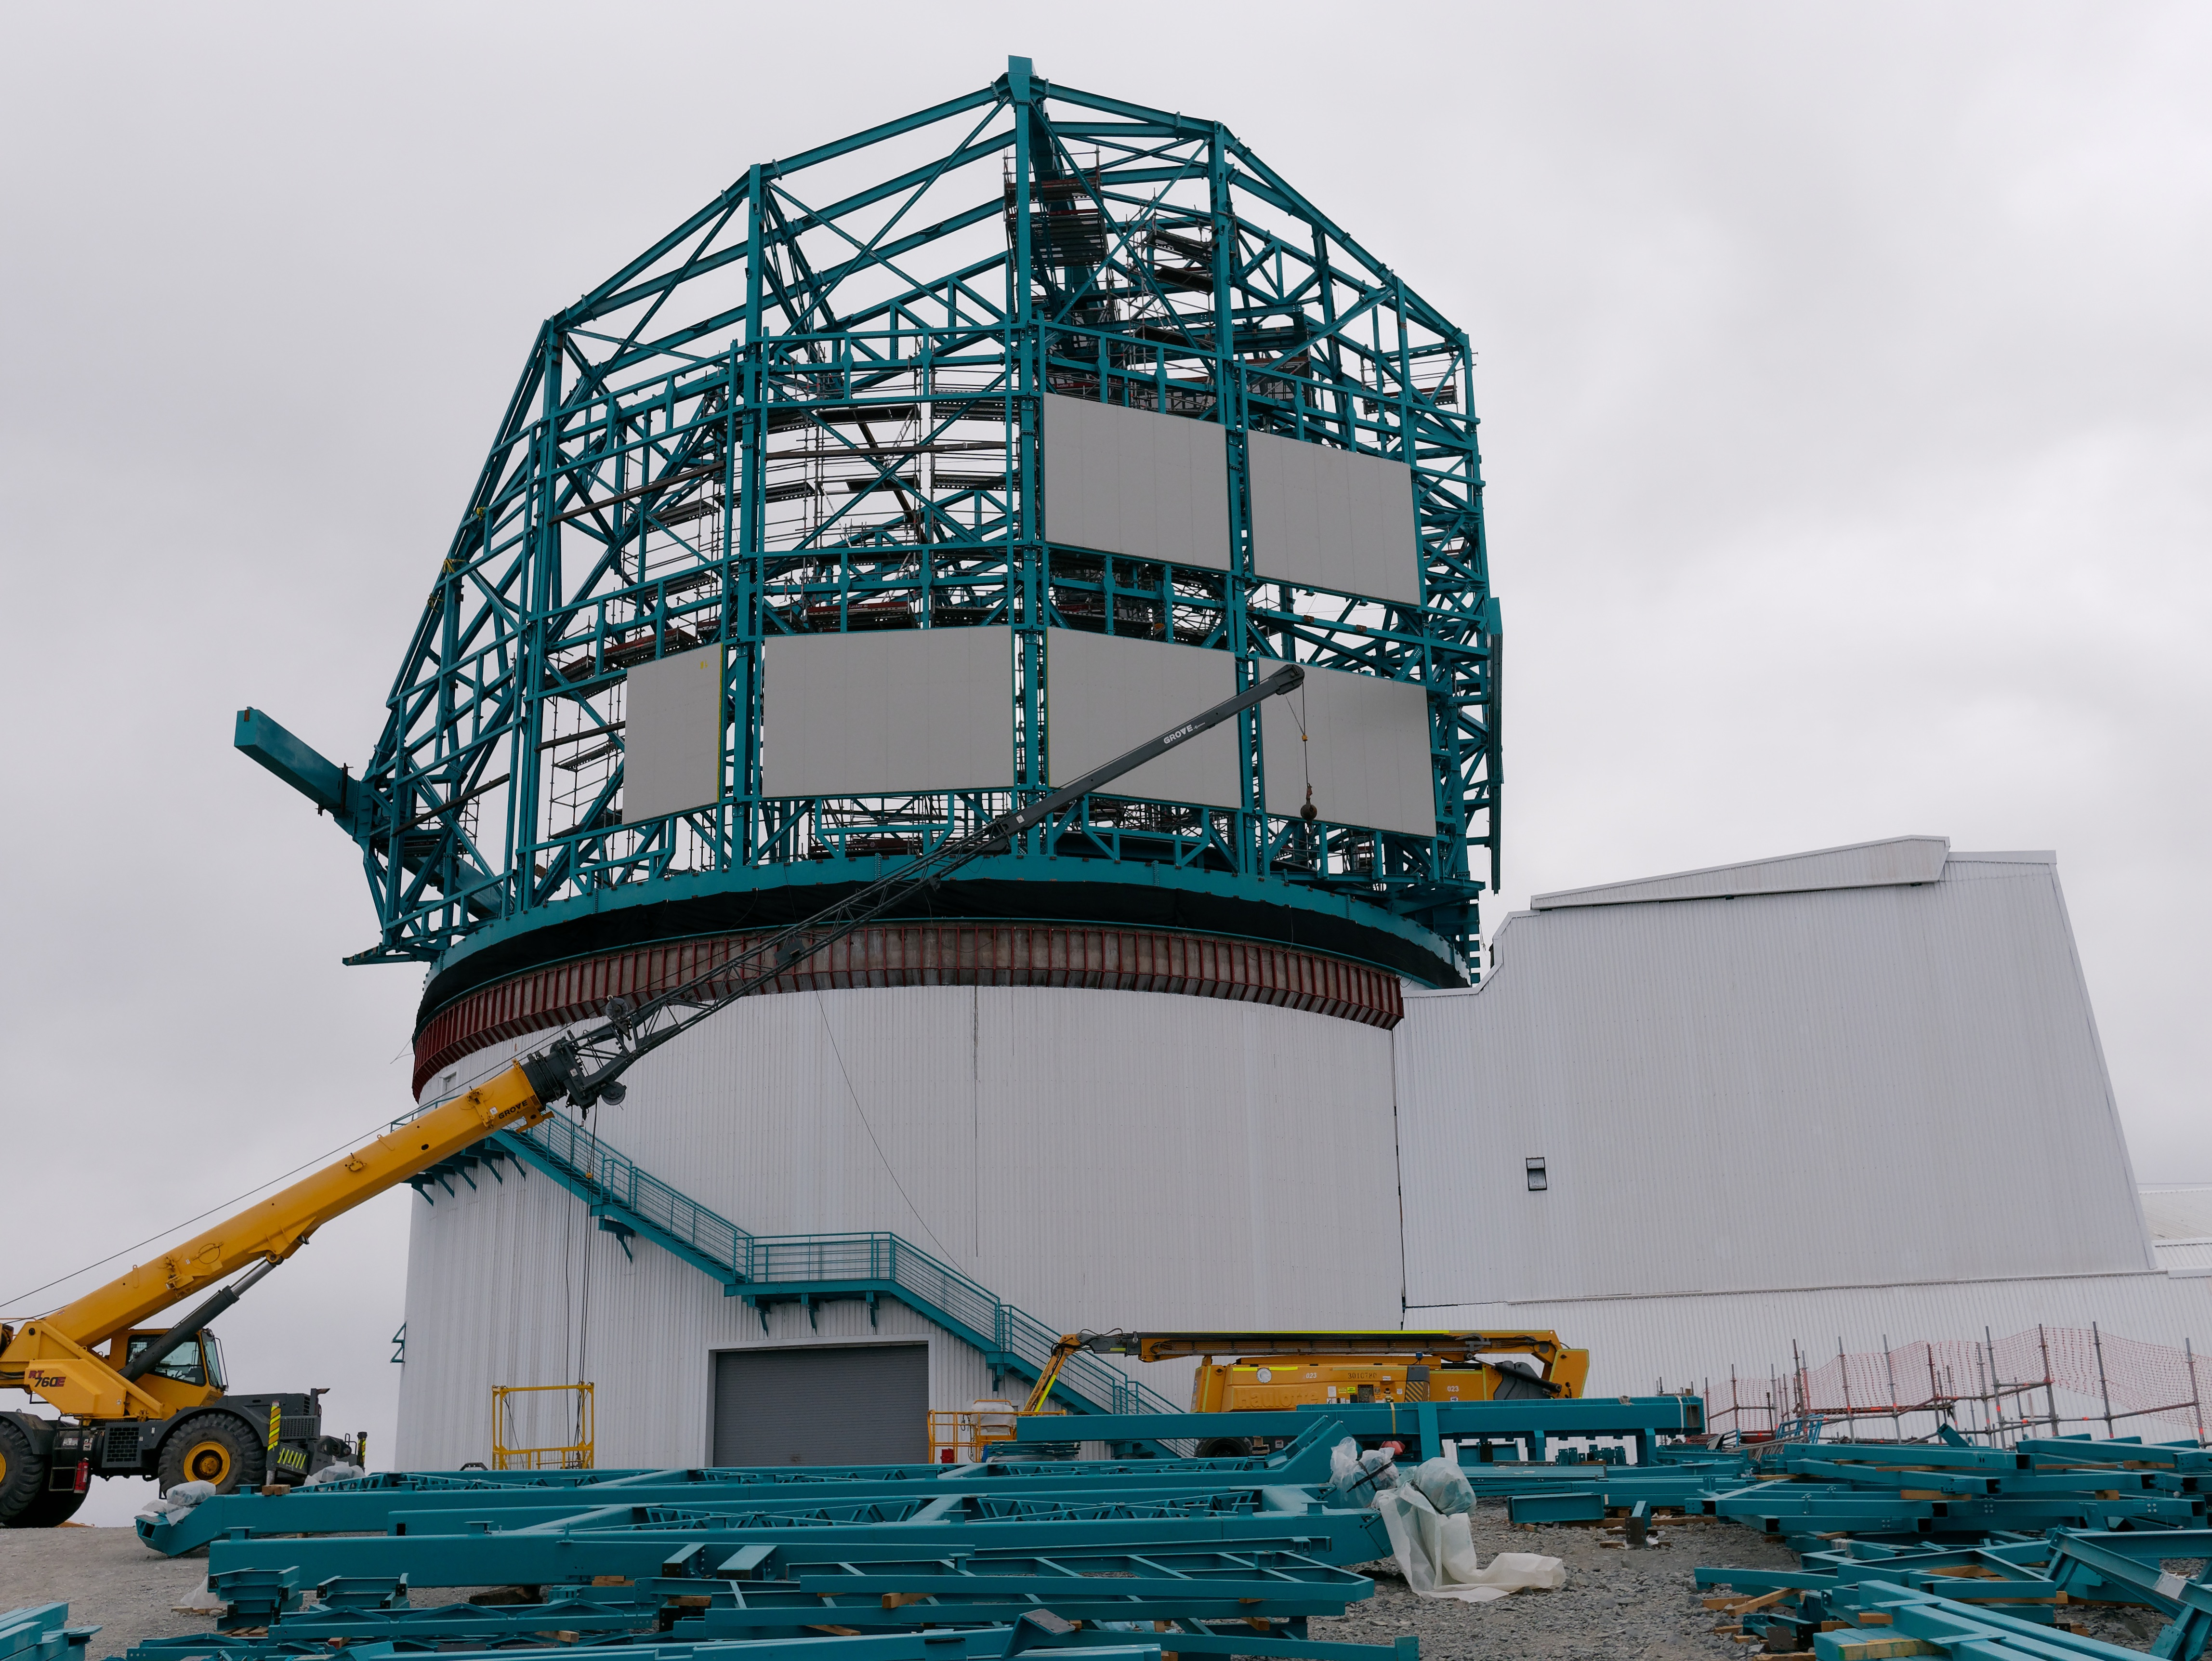
\includegraphics[width=0.6\textwidth]{lsst2019}
\end{center}
}


\frame{\frametitle{ Coating Chamber }
\begin{center}

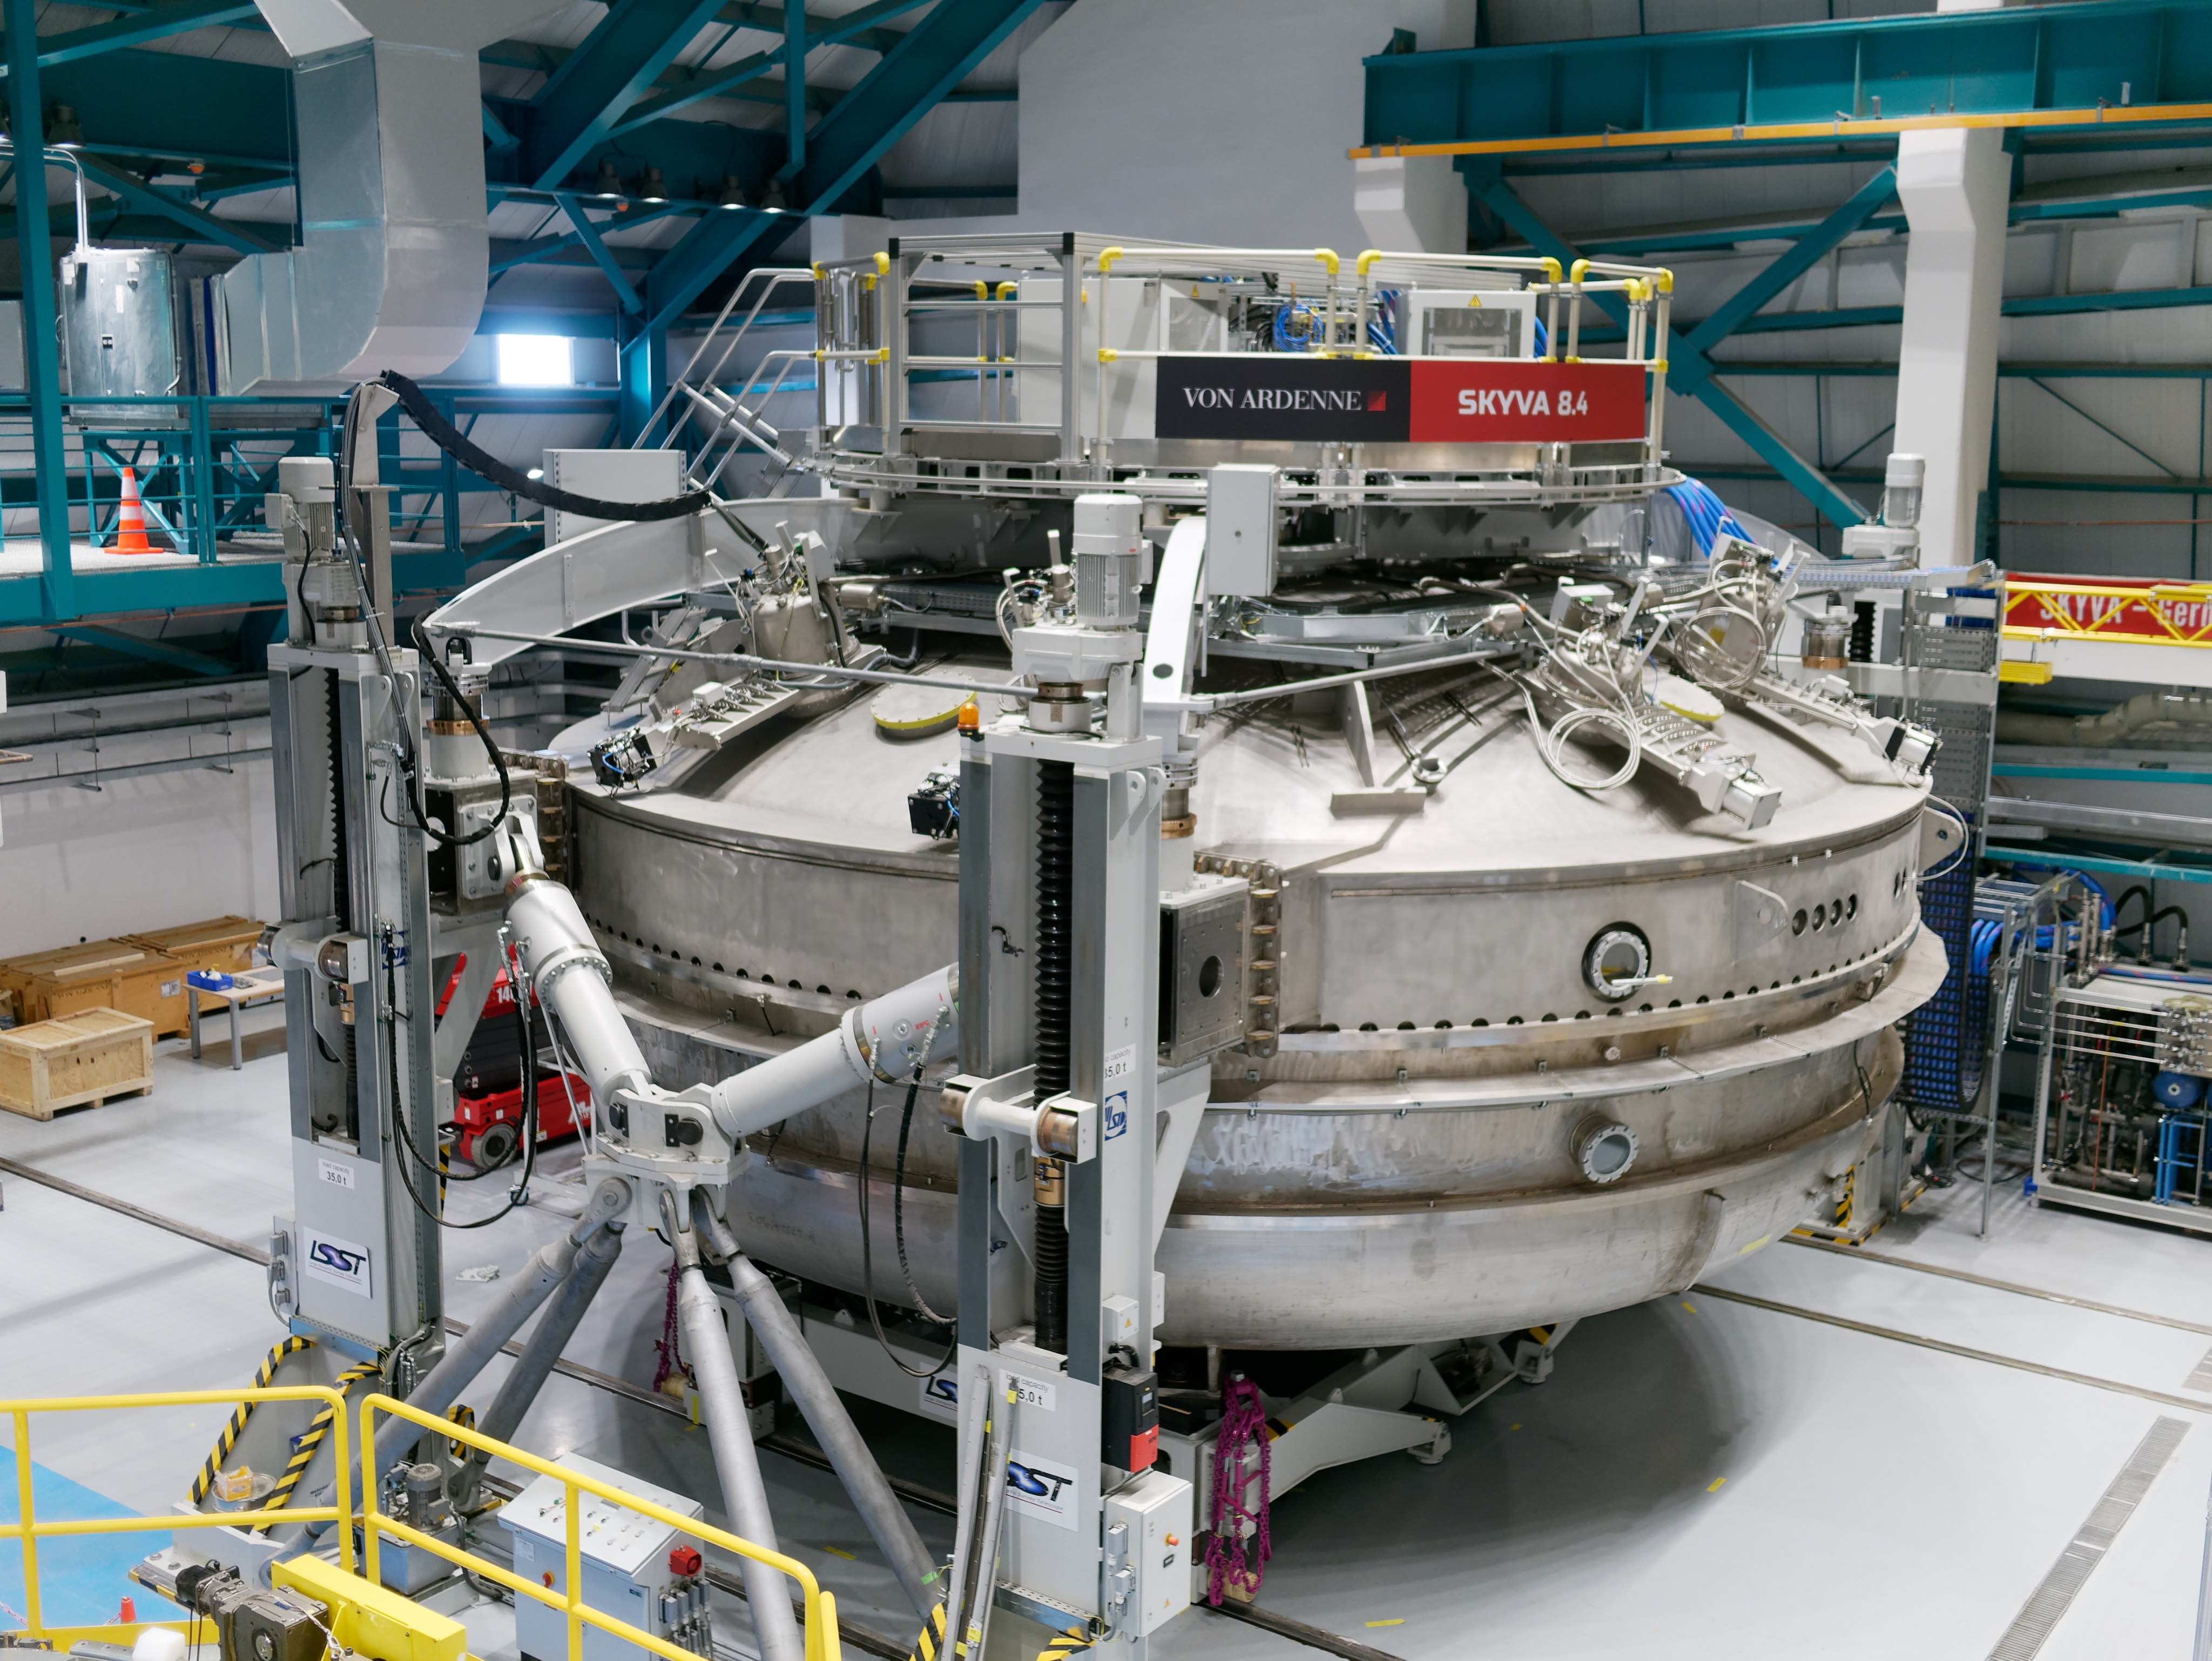
\includegraphics[width=0.6\textwidth]{cc2019}
\end{center}
}

\section{Data Management }

\frame {\frametitle{Mission Statement}
\begin{columns}
\column{0.65\textwidth}
      \includegraphics[width=1.0\textwidth]{images/DmMap}\\
\column{0.35\textwidth}
 \\
\vspace{-6.5cm}

DM's mission:\\
    \textit{Stand up operable, maintainable, quality services to deliver high-quality LSST data products for science, all on time and within reasonable cost.}\\
    \vspace{12pt}
Development is distributed across the Americas.\\

{\color{blue} Plus we have partners like IN2P3 (France).}\\
\vspace{8pt}
See the DM management plan, \citeds{LDM-294}.

\end{columns}
}


\frame {\frametitle{DM Organization}
\vspace{-0.5cm}
\begin{columns}
\column{0.73\textwidth}
\begin{center}
      \includegraphics[width=1.0\textwidth]{images/DmOrg}\\
\end{center}
\column{0.27\textwidth}

\vspace{0.4cm}
   Michelle Butler now NCSA TCAM \\ \smallskip
   DMCCB more active with weekly meetings\\ \smallskip
   SUIT is now dormant\\
   Roles etc in \citeds{LDM-294}\\

\end{columns}
}


\frame{\frametitle{New people - moving people}
\begin{itemize}
\item  Joining DM
\begin{itemize}
\item Lee Kelvin - joins DRP from Liverpool John’s Moore’s University
\item Arun Kannawadi - joins DRP from Leiden Observatory
\item Clare Saunders ( who can’t make PCW) - joins DRP  from “Laboratoire de Physique Nucl\'eaire et de Hautes \'Energies, IN2P3, CNRS
\end{itemize}
\item  Moving
\begin{itemize}
\item Jeff Carlin - moved to the DM Science  from Project Office
\item Hsin-fang Chang - moved from NCSA to AURA
\end{itemize}
\end{itemize}
}



\frame {\frametitle{Thank You !}
\vspace{-0.3cm}
\
\begin{columns}
\begin{column}{0.3\textwidth}
DM has been busy!\\ \smallskip
$\sim{}1$ million lines of code/comments (C++/Python/Java/JavaScript/Kotlin; see SPIE paper by \citealp{2018SPIE10707E..09J})\\
\end{column}
\begin{column}{0.7\textwidth}

\vspace{-1.3cm}
      \includegraphics[width=1.0\textwidth]{images/linesOfCode}\\
{\tiny \bf diagram by Tim Jenness; covers only the Science Pipelines codebase.}
\end{column}
\end{columns}
}

\frame{\frametitle{ DM indicators - Thank you all Again ! }
You may not care  much about these numbers but our funding agencies do.
\begin{center}
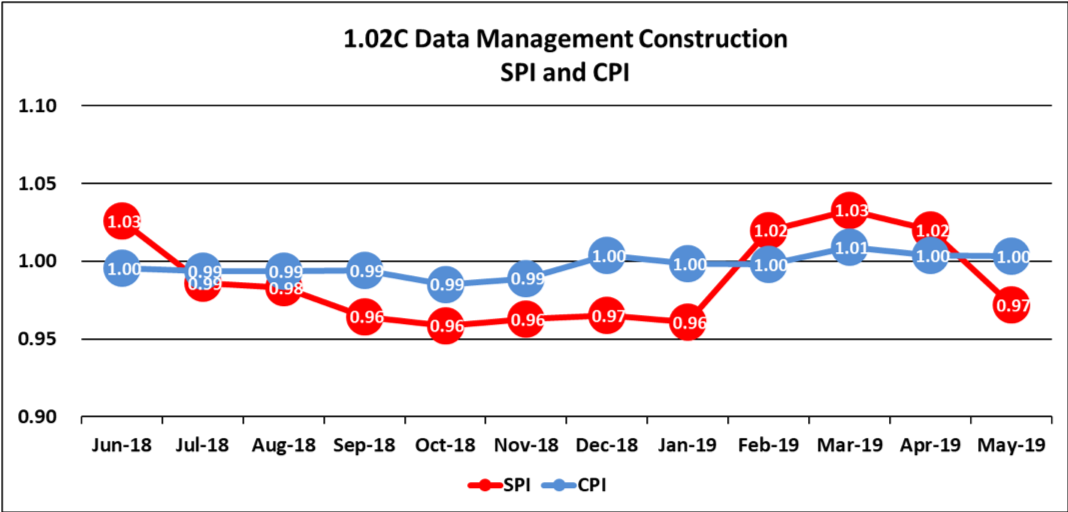
\includegraphics[width=0.8\textwidth]{figures/vari}
\end{center}
}




\frame{\frametitle{DM Verification Control Document}
\begin{itemize}
\item DM VCD available at \citeds{LDM-692}.
\begin{itemize}
\item Provides traceability from DM Requirements to Test Results
 through Verification Elements and Test Cases
\end{itemize}
\item DM Verification summary (from LDM-692 \S2):
\end{itemize}

\vspace{-9pt}
\centering
\small
\begin{longtable}{rrr}
&
\begin{tabular}{@{}l@{}} Num.\\Requirements \end{tabular} &
\begin{tabular}{@{}l@{}} Num. Verification\\Elements \end{tabular} \\ \hline\noalign{\smallskip}
Not related to any Test Case & 260 & 536 \\[0.1cm]
Related to NOT executed Test Cases & 352 & 384 \\[0.1cm]
Related to Failed Test Cases & 2 & 2 \\[0.1cm]
Related to Passed Test Cases & 79 & 80 \\[0.1cm]
\hline\noalign{\smallskip}
\textbf{Total} & \textbf{693} & \textbf{1002} \\
\end{longtable}
\vspace{-5pt}
There are 58 1a requirements which should be verifified for commissioning start.
}

\frame { \frametitle{High Level Goals}
 \begin{itemize}
   \item{Late 2019: Base Center Integration Complete}
   \item{Early 2020: Auxiliary Telescope Data Processing}
   \item{Early 2021: ComCam Data Processing}
   \item{Mid 2021: LSSTCam Data Processing}
   \item{Mid 2021: US Data Access Center Integrated}
 \end{itemize}
\vspace{-0.34cm}
 \begin{center}
 \textit{\citeds{LDM-564} describes the functionality provided at each milestone.\\Test plans to confirm milestone completion under development.}
 \end{center}
\vspace{-0.40cm}
\begin{center}
\small{
}
 \end{center}
}

\frame {
  \frametitle{Hyper Suprime Cam (HSC) on Subaru}
        \vspace{-3mm}
        \begin{columns}
                \column{0.5\textwidth}
              \begin{center}
              \includegraphics[width=0.9\textwidth]{images/HSCcosmos}\\
              \end{center}
                      \column{0.5\textwidth}
                       \\
                       \vspace{1cm}
                       HSC image (COSMOS) from g, r (1.5 hrs), and i (3 hrs) bands; PSF matched co-add ($\approx 27.5$).\\
                       \vspace{3mm}
                       Processed with the \textit{LSST Science Pipelines}\\\url{https://pipelines.lsst.io/}.\\
                       \vspace{3mm}
                       We regularly reprocess data from HSC and other precursor facilities at the LSST Data Facility as part of our integration tests.\\
                       \vspace{10mm}
               {\tiny \bf{Image courtesy of the HSC collaboration \& Robert Lupton}}
               \end{columns}

}





\frame{\frametitle{ Auxiliary Telescope \& LATISS}

\begin{center}
{\color{red} Early commissioning is coming soon! }
\end{center}

\begin{itemize}
\item The Auxiliary Telescope is operable already; the instrument --- LATISS (LSST Atmospheric Transmission Imager and Slitless Spectrograph) --- will arrive in October.
\begin{itemize}
\item Official operations imminent: milestone LDM-503-08 in preparation for that.
\end{itemize}
\item We have a pipeline for processing AuxTel image data.
\item We will shortly have a pipeline for LATISS data.
\item There will be a machine on the mountain for this processing (see also \citeds{DMTN-111}).
\item Initially \emph{selected} data will be transferred to NCSA and made available in the Science Platform.
\end{itemize}
}


\section{Some Highlights }

\frame{\frametitle{Science Team}

\begin{itemize}
  \item Workshops and Reviews:
  \begin{itemize}
      \item LSST Science Platform Final Design Review, Tucson, AZ 12-14 April 2019.
      \item Community Broker Workshop, ls.st/cbw, Seattle, WA 19-21 June 2019.
  \end{itemize}
\item Liaisons with Science Collaborations:
  \begin{itemize}
   \item Continual presence at ``Stack Club'' to support LSST scientists and understand user needs.
   \item Science Team liaisons to science collaborations attend meetings, workshops and present DM status.
 \end{itemize}
\item Verification and Validation:
  \begin{itemize}
    \item LSST Data Management Acceptance Test Specification \citeds{LDM-639}.
    \item One new FTE working on DM verification since December 2018.
    \item Science verification workshop --- a collaboration between Commissioning,  DM and Camera Subsystems --- took place in June 2019.
 \end{itemize}

\end{itemize}
}

\frame{{Alert Production}

      \begin{itemize}
        \item{Proof-of-concept design for scalable Alert Filtering Service (formerly ``mini-broker''); see \citeds{DMTN-093}.}
      \end{itemize}

  \vspace{-0.3cm}
  \begin{center}
    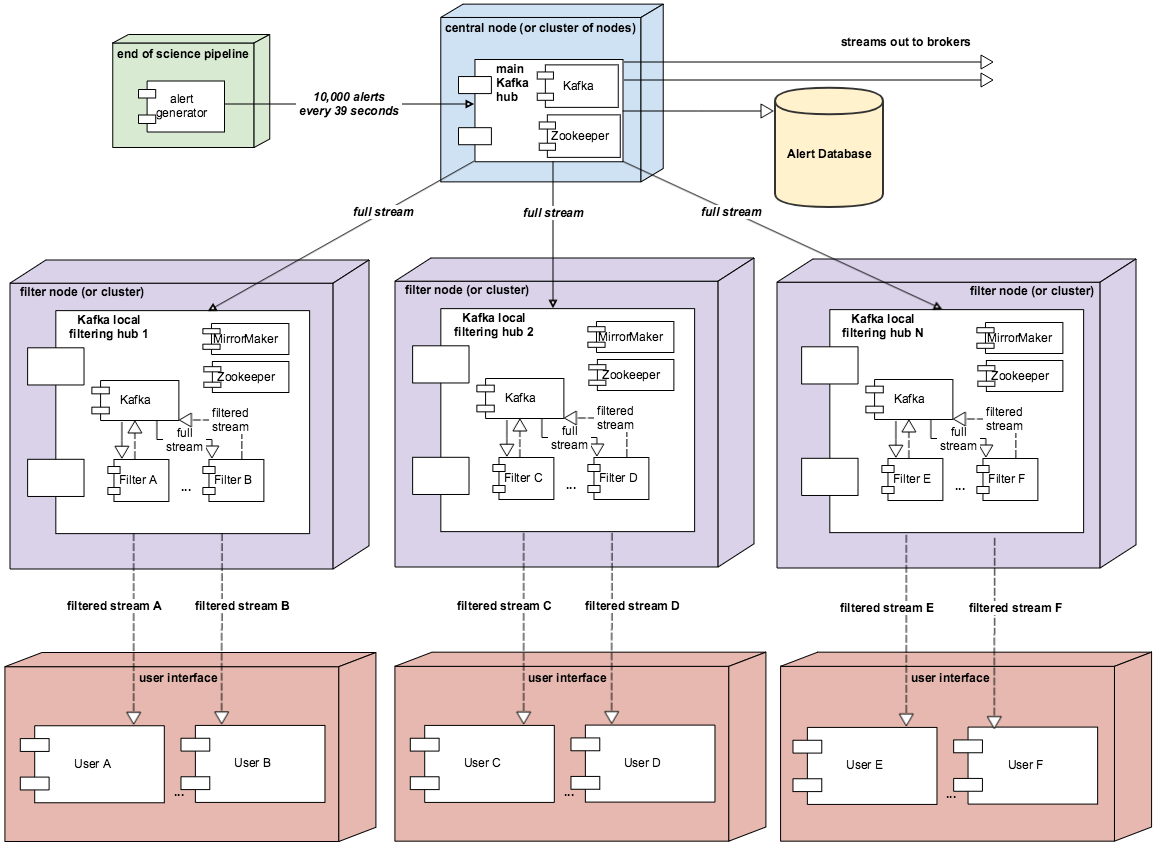
\includegraphics[width=0.5\textwidth]{figures/lafs.png}
  \end{center}
  \vspace{-0.7cm}
  \hspace{11.5cm}
  \tiny Figure: Patterson.

}

\frame{{Data Release Production}

  \begin{itemize}
   \item   {\textbf{LDM-503-07: Camera Data Processing}: Level 2 milestone demonstrating basic processing of data from \emph{physical LSST hardware} through Science Pipelines.}

        \item{The DRP team undertook a very successful ``sprint'' to integrate the SCARLET deblender \citep{2018A&C....24..129M} into the LSST Science Pipelines; it can now be run as part of regular LSST processing.}
            \item{The DRP team have integrated a version of the Forward Global Calibration Model \citep[FGCM;][]{2018AJ....155...41B} with the LSST Pipelines, and have extended it to provide absolute photometric calibration with respect to a reference catalog.}
 \item{A first prototype of the one-dimensional spectral extraction pipeline designed to reduce data produced by the Auxiliary Telescope Spectrograph has been produced.}
           \item{Delivered partial mitigation for the brighter-fatter effect \citep{2014JInst...9C3048A}.}

  \end{itemize}

}

\frame{\frametitle{Base \& Network}
\begin{itemize}
\item Demonstrated 100\,Gbps from Base to NCSA in November at Supercomputing 2018.
\item 10\,TB of DECam data via SCInet via Miami -- Dallas -- Chicago.
\item Jupyter notebook used to monitor process from Data Transfer Node to disk at NCSA.
\end{itemize}
\centering
\vspace{-0.5cm}
\includegraphics[width=0.8\textwidth]{NetConfig2018}
}


\frame{\frametitle{Data Access Services}
\vspace{-0.2cm}

\begin{columns}
    \begin{column}{0.6\textwidth}
        \begin{itemize}
            \item Catalog Database (Qserv):
                \begin{itemize}
                   \item Currently hosting $\approx$ 175 TB across 30 nodes.
                     \begin{itemize}
                        \item NCSA: science dataset (Stripe 82 + WISE; Gaia DR2 soon).
                        \item CC-IN2P3: synthetic datasets.
                    \end{itemize}
                    \item Will scale to 75\% LSST DR1 by late 2019.
                    \item Cloud Deployment Demonstration \citedsp{DMTN-125}.
                    \begin{itemize}
                        \item Within 10-15\% perf. vs. dedicated hardware.
                    \end{itemize}
                \end{itemize}
            \item Web Services for Science Platform:
                \begin{itemize}
                    \item Built around IVOA standards.
                    \item TAP/ADQL query service (backed by Qserv) now online.
                    \item SODA image cutout service now online.
                    \item AstroPy PyVO Python client library improvements.
                \end{itemize}

        \end{itemize}
    \end{column}
    \begin{column}{0.4\textwidth}
        \begin{center}
            
\includegraphics[width=\columnwidth]{figures/qserv-in2p3.png}
        \end{center}
    \end{column}
\end{columns}

}


\frame{\frametitle{LSST Data Facility (NCSA)}

\begin{itemize}
\item L2 Milestones completed: LDM-503-8b, LDM-503-8, LDM-503-4, LDM-503-4b.  % Would be good to say what these actually are!

\item Spectrograph integration tests, culminating in running prompt forwarder \& archiver processes on LATISS test stand in Tucson. Data is made available in ``Butler'' repositories at the Data Facility (caveat not optimal nor final).
\item Delivered multiple services: Kubernetes, Qserv, HTCondor. Plus authorization \& authentication support to LSST  in Chile.
\item Demonstrated Pegasus Workflow Management System (on HTCondor) and ``Butler'' based on an Oracle database running with ``Generation 3'' DM middleware. Since decided to go direct to HTCondor (dropping Pegasus).
\item Integrated of Camera Data Acquisition hardware on the L1 Test Stand at NCSA; provided a tutorial on the new software interface.
\item Led Operations Rehearsal \#1 to prepare for commissioning by simulating nominal operations during a three-day observation period.
\item Procured and configured test systems for ComCam; supplied to Tucson.

\end{itemize}
}

\frame{\frametitle{SQuaRE}

\begin{itemize}
  \item Notebook Aspect of the Science Platform now well established.
  \item New InfluxDB back-end for the SQuaSH (metrics curation) service.
  \item Also new: automated report creation from notebook templates.
  \item Prototyped DM Engineering \& Facility Database based on Kafka \& InfluxDB; demonstrated impressive scaling to 50\,Hz.

\end{itemize}
\begin{center}
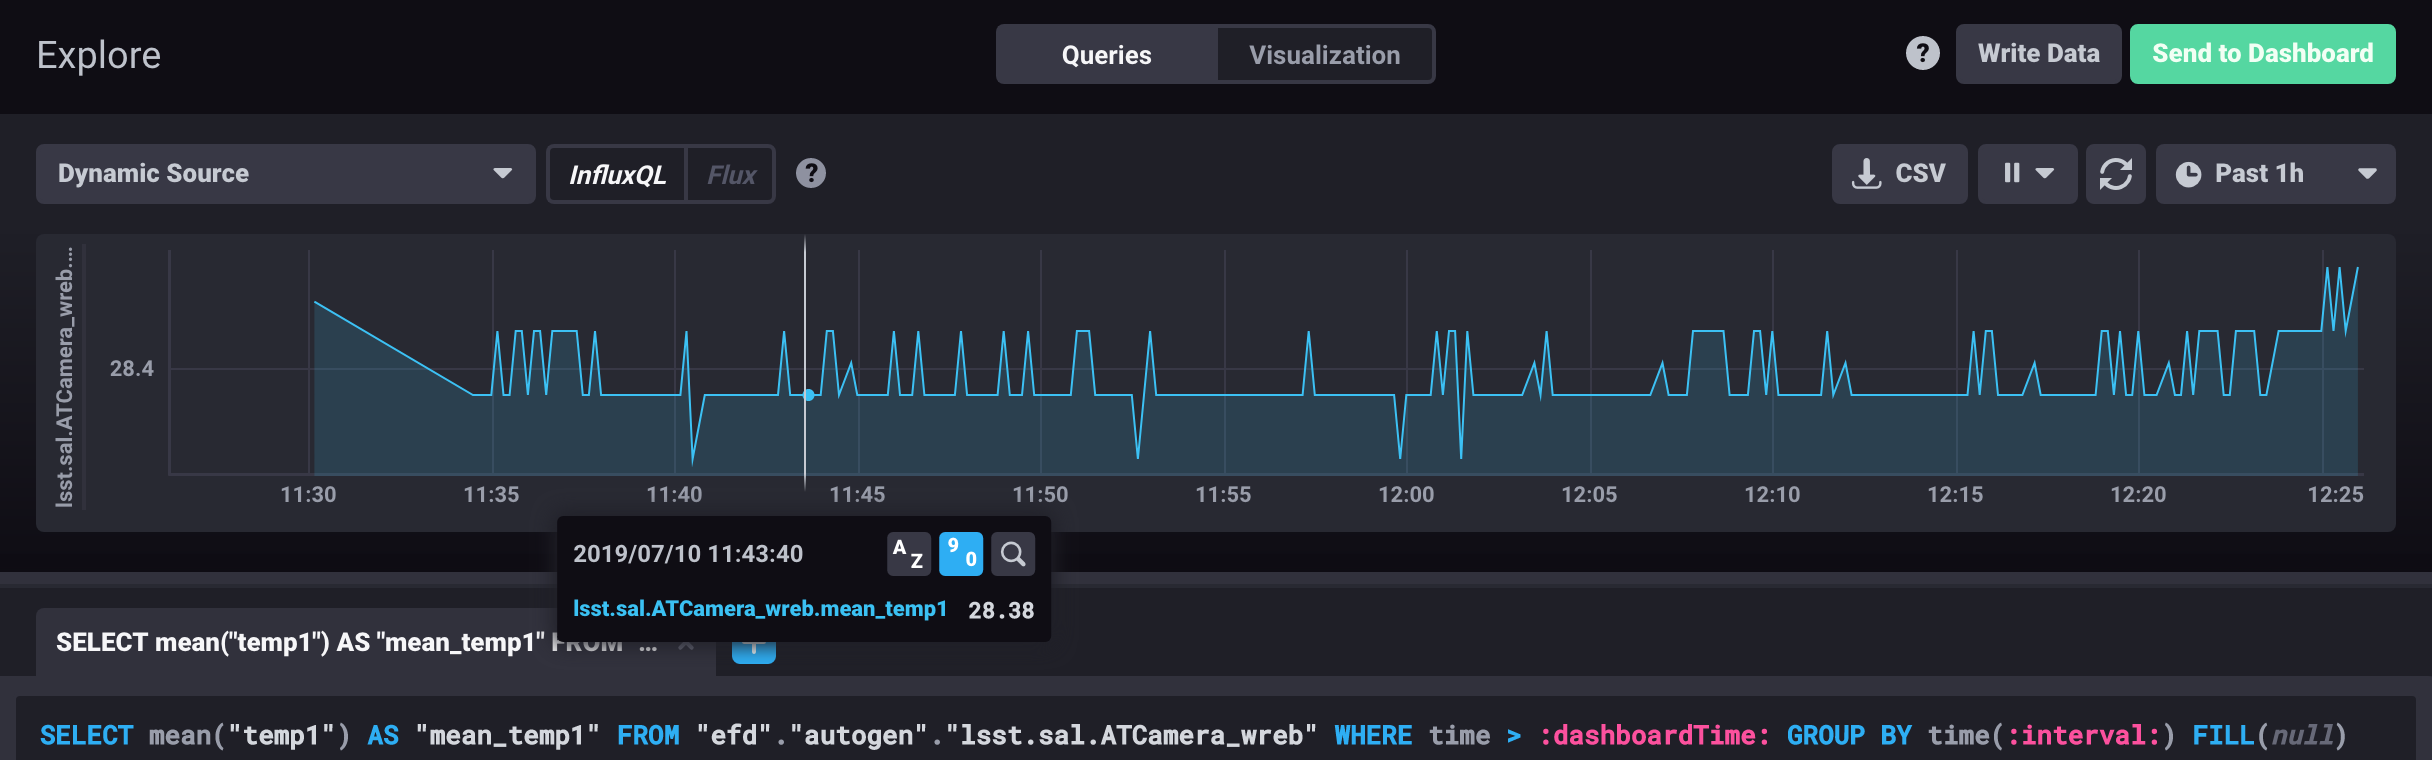
\includegraphics[width=0.8\textwidth]{figures/efd-live}
\end{center}
}

\frame {
  \frametitle{Hyper Suprime Cam (HSC) on Subaru}
        \vspace{-3mm}
        \begin{columns}
                \column{0.5\textwidth}
              \begin{center}
              \includegraphics[width=0.9\textwidth]{images/HSCcosmos}\\
              \end{center}
                      \column{0.5\textwidth}
                       \\
                       \vspace{1cm}
                       HSC image (COSMOS) from g, r (1.5 hrs), and i (3 hrs) bands; PSF matched co-add ($\approx 27.5$).\\
                       \vspace{3mm}
                       Processed with the \textit{LSST Science Pipelines}\\\url{https://pipelines.lsst.io/}.\\
                       \vspace{3mm}
                       We regularly reprocess data from HSC and other precursor facilities at the LSST Data Facility as part of our integration tests.\\
                       \vspace{10mm}
               {\tiny \bf{Image courtesy of the HSC collaboration \& Robert Lupton}}
               \end{columns}

}



\frame{\frametitle{ Reviews}
\begin{itemize}

\item{Just finished Joint Directors Review - 2 recommendations
  \begin{itemize}
    \item{ More cloud. }
    \item{ tooling for workflows especially debugging .}
	\item {General feed back was positive.}
  \end{itemize}
}
\item{Joint status review end of the month. }


\end{itemize}
}


\frame{\frametitle{ Exploring possibilities}
\begin{itemize}
\item Google
\begin{itemize}
\item Initial cost estimates based on a simplified sizing model (\citeds{DMTN-072}) formed basis.
\item Report in \citeds{DMTN-125} --- highlights include:
\begin{itemize}
\item Deployed Qserv on Google with reasonable performance (80\% or better of in-house)
\item Data transfer adequate for Prompt Processing demonstrated, within the limits of the available network. Prompt Product Database stood up and tested.
\item Science Platform deployed and users simulated.
\end{itemize}
\item Successfully viability of the ideas, but more effort would be required to take this further.
\end{itemize}
\item AWS
\begin{itemize}
\item Processing with Amazon Web Services / Elastic Compute Cloud and HTCondor.
\item Investigation currently underway, being lead by Hsin-Fang Chiang (NCSA).
\item See \citeds{DMTN-114} for details --- goals include:

\begin{itemize}
\item Demonstrate HSC data processing test on Amazon, integrated with their S3 object storage system; ultimately, scale to large data volumes.
\item Stretch: Reprocess DESC DC2.
\item Stretch: Offer tutorial at \href{https://petabytestoscience.github.io/workshop-iii}{Data Inclusion Revolution in Boston in November}
\end{itemize}
\end{itemize}
\end{itemize}
}

\frame{\frametitle{Transition to Operations}
\begin{itemize}
\item In Operations, the DM will transition into the Science Operations and Data Facility directorates.
\item We have identified specific roles within those directorates which will be filled by current DM staff.
\item We expect that DM staff who wish to transition to operations should be able to do so, although we're still in the process of figuring out roles and locations.
\item A few people will begin transitioning to the pre-operations budget next year.
\end{itemize}
}

\section{Conclusion}

\frame{\frametitle{Conclusion}
\begin{itemize}
\item DM is functioning and following the plan.
\item Your efforts are appreciated - DM is now seen in good light in reviews.
\item The project is moving ahead rapidly - expect more issues as we get closer to reality.
\item Enjoy Hoodies - Photo at end of this session !
\item DM Night out on Wednesday - partners welcome.

\end{itemize}
}

\frame { \frametitle{ The END }
\vspace{-0.3cm}
\begin{center}
 \includegraphics[width=0.5\textwidth]{images/EIA-TUCSON-2018.jpg}
\vspace{-3.5cm}\hspace{0.6cm} \huge{\color{red} Questions?}\\
\vspace{+3.6cm}
\normalsize
{\tiny Image: Early Integraiton in Tucson 2018 with Jim Parsons$^{\dag}$}
\end{center}

}




\appendix

\section {Reference material}
\frame[allowframebreaks]{\frametitle{ Acronyms }
        \vspace{10pt}
        \tiny
        \addtocounter{table}{-1}
\begin{longtable}{|p{0.145\textwidth}|p{0.8\textwidth}|}\hline
\textbf{Acronym} & \textbf{Description}  \\\hline

ADQL & Astronomical Data Query Language \\\hline
AURA & Association of Universities for Research in Astronomy \\\hline
AWS & Amazon Web Services \\\hline
Alert & A packet of information for each source detected with signal-to-noise ratio > 5 in a difference image during Prompt Processing, containing measurement and characterization parameters based on the past 12 months of LSST observations plus small cutouts of the single-visit, template, and difference images, distributed via the internet \\\hline
Alert Production & The principal component of Prompt Processing that processes and calibrates incoming images, performs Difference Image Analysis to identify DIASources and DIAObjects, packages and distributes the resulting Alerts, and runs the Moving Object Processing System \\\hline
BAC & Budget At Complete \\\hline
Broker & Software which receives and redistributes Alerts, and may also perform processing such as filtering for certain characteristics, cross-matching with non-LSST catalogs, and/or light-curve classification, in order to identify and prioritize targets for follow-up and/or make scientific analyses.  \\\hline
Butler & A middleware component for persisting and retrieving image datasets (raw or processed), calibration reference data, and catalogs \\\hline
CC & Change Control \\\hline
CCOB & Camera Calibration Optical Bench \\\hline
Camera & The LSST subsystem responsible for the 3.2-gigapixel LSST camera, which will take more than 800 panoramic images of the sky every night. SLAC leads a consortium of Department of Energy laboratories to design and build the camera sensors, optics, electronics, cryostat, filters and filter exchange mechanism, and camera control system \\\hline
Center & An entity managed by AURA that is responsible for execution of a federally funded project \\\hline
DM & Data Management \\\hline
DMCCB & DM Change Control Board \\\hline
DMTN & DM Technical Note \\\hline
DMTR & DM Test Report \\\hline
DRP & Data Release Production \\\hline
Data Access Center & Part of the LSST Data Management System, the US and Chilean DACs will provide authorized access to the released LSST data products, software such as the Science Platform, and computational resources for data analysis. The US DAC also includes a service for distributing bulk data on daily and annual (Data Release) timescales to partner institutions, collaborations, and LSST Education and Public Outreach (EPO).  \\\hline
Data Management & The LSST Subsystem responsible for the Data Management System (DMS), which will capture, store, catalog, and serve the LSST dataset to the scientific community and public. The DM team is responsible for the DMS architecture, applications, middleware, infrastructure, algorithms, and Observatory Network Design. DM is a distributed team working at LSST and partner institutions, with the DM Subsystem Manager located at LSST headquarters in Tucson \\\hline
Data Release Production & An episode of (re)processing all of the accumulated LSST images, during which all output DR data products are generated. These episodes are planned to occur annually during the LSST survey, and the processing will be executed at the Archive Center. This includes Difference Imaging Analysis, generating deep Coadd Images, Source detection and association, creating Object and Solar System Object catalogs, and related metadata \\\hline
Document & Any object (in any application supported by DocuShare or design archives such as PDMWorks or GIT) that supports project management or records milestones and deliverables of the LSST Project \\\hline
FGCM &  Forward Global Calibration Model \\\hline
FTE & Full Time Equivalent \\\hline
HSC & Hyper Suprime-Cam \\\hline
IVOA & International Virtual-Observatory Alliance \\\hline
LATISS & LSST Atmospheric Transmission Imager and Slitless Spectrograph \\\hline
LDM & LSST Data Management (Document Handle) \\\hline
LSST & Large Synoptic Survey Telescope \\\hline
NCSA & National Center for Supercomputing Applications \\\hline
OPS & Operations \\\hline
Offer & A response to a solicitation that, if accepted, would bind the offeror to perform the work described in resultant contract. Responses to sealed bidding are offers that are often referred to as 'bids' or 'sealed bids;' responses to a request for proposals (RFP, negotiated-type procurements) are offers often referred to as 'proposals' responses to a request for quotations (RFQ) are not offers and are generally called 'quotes' \\\hline
Operations & The 10-year period following construction and commissioning during which the LSST Observatory conducts its survey \\\hline
Operations Rehearsal & A data management system prototype project employing the same methods, tools, personnel, and technologies as the real system in order to introduce and validate new algorithms, functionality, and infrastructure. Previously referred to as a data challenge \\\hline
PCW & Project Community Workshop \\\hline
PSF & Point Spread Function \\\hline
Project Manager & The person responsible for exercising leadership and oversight over the entire LSST project; he or she controls schedule, budget, and all contingency funds \\\hline
Prompt Processing & The processing that occurs at the Archive Center on the nightly stream of raw images coming from the telescope, including Difference Imaging Analysis, Alert Production, and the Moving Object Processing System. This processing generates Prompt Data Products \\\hline
Qserv & Proprietary Database built by SLAC for LSST \\\hline
Release & Publication of a new iteration of an existing document following approval of changes through the change control process. Upon release, the new iteration becomes the current baseline and the preferred version in the archive \\\hline
Review & Programmatic and/or technical audits of a given component of the project, where a preferably independent committee advises further project decisions, based on the current status and their evaluation of it. The reviews assess technical performance and maturity, as well as the compliance of the design and end product with the stated requirements and interfaces \\\hline
SODA & Server-side Operations for Data Access \\\hline
SPIE & The international society for optics and photonics \\\hline
SQuaRE & Science Quality and Reliability Engineering \\\hline
SQuaSH & Science Quality Analysis Harness \\\hline
SUIT & Science User Interface and Tools \\\hline
Science Pipelines & The library of software components and the algorithms and processing pipelines assembled from them that are being developed by DM to generate science-ready data products from LSST images. The Pipelines may be executed at scale as part of LSST Prompt or Data Release processing, or pieces of them may be used in a standalone mode or executed through the LSST Science Platform. The Science Pipelines are one component of the LSST Software Stack \\\hline
Science Platform & A set of integrated web applications and services deployed at the LSST Data Access Centers (DACs) through which the scientific community will access, visualize, and perform next-to-the-data analysis of the LSST data products \\\hline
Specification & One or more performance parameter(s) being established by a requirement that the delivered system or subsystem must meet \\\hline
Stripe 82 & A 2.5° wide equatorial band of sky covering roughly 300 square degrees that was observed repeatedly in 5 passbands during the course of the SDSS, In part for calibration purposes \\\hline
TAP & Table Access Protocol \\\hline
TB & TeraByte \\\hline
TCAM & Technical Control (or Cost) Account Manager \\\hline
US & United States \\\hline
VCD & Verification Control Document \\\hline
Validation & A process of confirming that the delivered system will provide its desired functionality; overall, a validation process includes the evaluation, integration, and test activities carried out at the system level to ensure that the final developed system satisfies the intent and performance of that system in operations \\\hline
Verification & The process of evaluating the design, including hardware and software - to ensure the requirements have been met;  verification (of requirements) is performed by test, analysis, inspection, and/or demonstration \\\hline
WISE & Wide-field Survey Explorer \\\hline
brighter-fatter effect & The common term used to refer to one of the photometric qualities of the LSST camera: sources with a higher flux have a broader PSF. This is accounted for during calibration \\\hline
calibration & The process of translating signals produced by a measuring instrument such as a telescope and camera into physical units such as flux, which are used for scientific analysis. Calibration removes most of the contributions to the signal from environmental and instrumental factors, such that only the astronomical component remains \\\hline
pipeline & A configured sequence of software tasks (Stages) to process data and generate data products. Example: Association Pipeline \\\hline
\end{longtable}

}

\frame[allowframebreaks]{\frametitle{ References }
       \tiny
       \bibliographystyle{lsst_aa}
       \bibliography{local,lsst,gaia_livelink_valid,refs,books,refs_ads}
       \normalsize

}



\end{document}
